\section{Theorie}
\label{sec:Theorie}
Die Beugung des Lichts beschreibt das Phänomen, dass die Lichtausbreitung von den Gesetzen der geometrischen Optik abweicht, wenn ein Lichtstrahl auf Öffnungen trifft, deren Abmessung klein gegen den Durchmesser des Lichtstrahls ist. Gut erklären lässt sich dies, indem das Licht als Welle aufgefasst wird, was aufgrund der großen Anzahl an Photonen hier als Näherung verwendet werden kann. 

Grundsätzlich gibt es zwei Ansätze für Beugung am Spalt, die Fresnelsche und die Fraunhofersche Beugung (s. Abb. \ref{fig:frauenhoferfresnel}). 

\begin{figure}[h!]
	\centering
	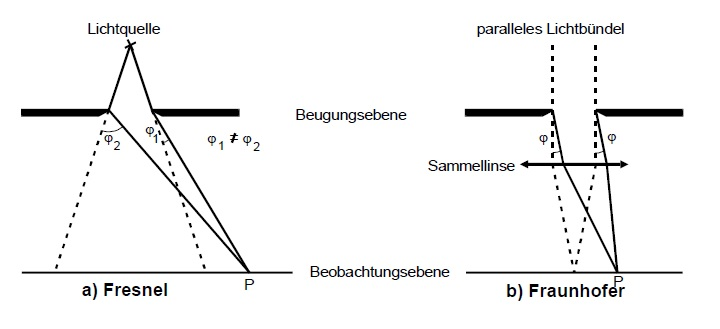
\includegraphics[width=0.9\linewidth]{../../FrauenhoferFresnel}
	\caption{Beugung nach Fresnel und Fraunhofer an einem Spalt, \cite[2]{anleitung406}.}
	\label{fig:frauenhoferfresnel}
\end{figure}

Fresnel geht von einer Lichtquelle in endlicher Entfernung vom Spalt aus, sodass sich eine divergente Lichtausbreitung ergibt. Das ist auch in der Abbildung \ref{fig:frauenhoferfresnel} zu sehen. Es hat zur Folge, dass die Strahlen, die im Punkt P beobachtet werden, unter verschiedenen Winkeln gebrochen werden. Die Fraunhofer Beugung geht hingegen von einer Lichtquelle im Unendlichen aus, wodurch sich ein paralleles Lichtbündel mit ebenen Wellenfronten ergibt. Dies hat den Vorteil, das es nur einen Brechungswinkel gibt und sich so die Auswertung des Versuches vereinfacht. Im Folgenden wird nur die Frauenhoferschen Beugung betrachtet, da ihre mathematische Beschreibung viel leichter ist. 

Das Huygenssche Prinzip geht nun davon aus, dass von jedem Punkt einer Wellenfront zur gleichen Zeit Elementarwellen kreisförmig auslaufen. Diese theoretisch unendlich vielen Wellen interferieren miteinander und bilden so neue Wellenfronten, die sich als Einhüllende der Elementarwellen betrachten lassen. 

\subsection{Beugung am Einzelspalt}
Wenn das Huygen-Fresnelsche Prinzip auf dem Einzelspalt übertragen wird, dann ist es zu erkennen, dass von jedem Punkte der Spaltöffnungen Kugelwellen ausgehen, die in alle Richtungen fortschreiten. Somit muss dann auch über alle Strahlbündel summiert werden, die unter dem Winkel $\varphi$ abgelenkt werden, um die Amplitude in $\varphi$-Richtung zu berechnen. Allerdings stellt es sich fest, dass die Wellenfronten der Strahlbündel sehr klein sind. Zum einen wird davon ausgegangen, dass eine Welle sich über die Gleichung:
\begin{equation}
A(z,t) = A_0 \cdot \text{exp}\{i(wt-2s\pi/\lambda)\}
\end{equation}
beschreiben lässt. Gehen von jedem Punkt der Spaltöffnung sich in alle Richtungen ausbreitende Wellen aus, ergeben sich aus der Interferenz Maxima und Minima der Lichtintensität.
\begin{figure}[h!]
	\centering
	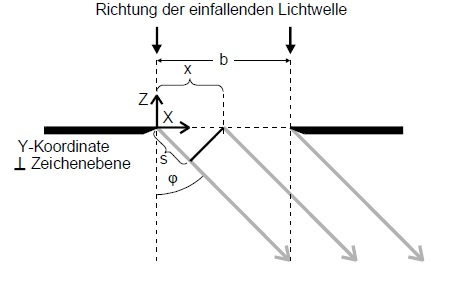
\includegraphics[width=0.9\linewidth]{../../BeugungamEinzelspalt}
	\caption{Beugung am Einzelspalt mit der Frauenhofscher Methode, \cite[3]{anleitung406}.}
	\label{fig:beugungameinzelspalt}
\end{figure}
Zum anderen werden zwei dieser Punkte im Abstand $x$ am Spalt genommen, sodass es sich durch ihren Gangunterschied $s$ die Phasendifferenz  $\delta$ ergibt(s. Abb. \ref{fig:beugungameinzelspalt}):
\begin{align}
\delta = \frac{2\pi s}{\lambda} = \frac{2\pi x\sin\varphi}{\lambda}
\end{align}
Dabei muss dieser Phasenunterschied bei der Summation berücksichtigt werden. Die Integration über die Spaltbreite $b$ der Funktion für die Amplitude $B$ in $\varphi$-Richtung:
\begin{align}
B(z,t,\varphi)=A_0 \int_0^b \exp\left\{i\left(\omega t - \frac{2\pi z}{\lambda} + \delta\right)\right\}dx
\end{align} 
($A_0$ ist die Amplitude der einfallenden Welle, z die Ausbreitungsrichtung und $\omega$ die Frequenz) ergibt mit Vernachlässigung der Phasenfunktionen:
\begin{align}
B(\varphi)=A_0 b \frac{\sin\eta}{\eta}\\
\eta=\frac{\pi b \sin\varphi}{\lambda}\text{.} 
\end{align} 
Die Funktion ist in der Abbildung \ref{fig:interferenzmustereinzelspalt} zu sehen. Da es sich um eine gerade Funktion handelt, die lokale Maxima und Minima sowie unendlich vielen Nulldurchgängen enthält, dann besitzt sie auch die Nullstellen bei:
\begin{equation}
\text{sin}(\varphi) = \pm n\frac{\lambda}{b}
\end{equation}
mit $n= 1,2,...$.

\begin{figure}[h!]
	\centering
	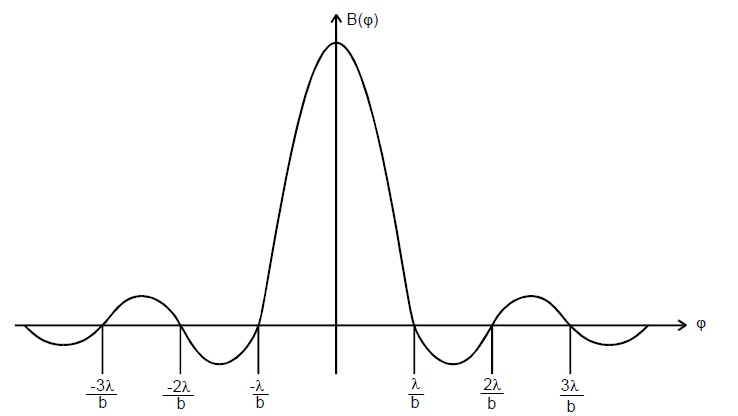
\includegraphics[width=0.9\linewidth]{../../InterferenzmusterEinzelspalt}
	\caption{Die Amplitude einer ebenen Welle am Parallelspalt, \cite[4]{anleitung406}.}
	\label{fig:interferenzmustereinzelspalt}
\end{figure}

Aufgrund der hohen Frequenzen im Bereich $\omega = \SI{E14}{\Hz}$ bis $\SI{E15}{\Hz}$ ist die Amplitude nicht direkt messbar. Man misst deshalb die zeitlich gemittelte Intensität $I(\varphi)$ des gebeugten Lichts. Diese ist bei am Parallelspalt gebeugten Licht gegeben durch:
\begin{align}
I(\varphi) \propto B(\varphi)^2 = A_0^2 b^2 \left\{\frac{\lambda}{\pi b\sin\varphi}\right\}^2\cdot\sin^2\left\{\frac{\pi b\sin\varphi}{\lambda}\right\}\text{.} \label{eq5}
\end{align}

\subsection{Beugung am Doppelspalt}
Wie beim Einzelspalt lässt sich analog die Intensitätsverteilung $I(\varphi)$ bestimmen. Die Beugung am Doppelspalt ist in der Abbildung \ref{fig:beugungamdoppelspalt} zu sehen. Die Beschreibung der Beugung am Doppelspalt erfolgt als Überlagerung zweier Einfach-Spalte mit Breite $b$ und Abstand $s$:
\begin{align}
I(\varphi) \propto B(\varphi)^2 = 4 A_{0}^{2} b^{2}\cos^2\left(\frac{\pi s\sin\varphi}{\lambda}\right)\left(\frac{\lambda}{\pi b \sin\varphi}\right)^2\sin^2\left(\frac{\pi b\sin\varphi}{\lambda}\right)\text{.}
\end{align}
\begin{figure}[h!]
	\centering
	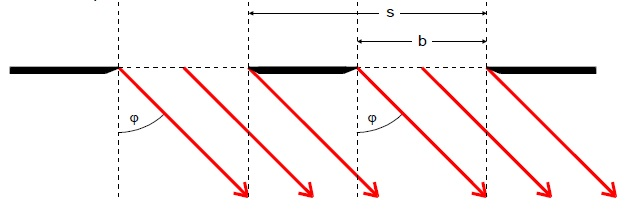
\includegraphics[width=0.9\linewidth]{../../BeugungamDoppelspalt}
	\caption{Beugung am Doppelspalt, \cite[4]{anleitung406}.}
	\label{fig:beugungamdoppelspalt}
\end{figure}
Es ergibt sich somit für den Doppelspalt die Intensitätsverteilung des Einzelspalts mit einem $\cos^2$-Term, wodurch sich zusätzlich Minima an den Nullstellen der $\cos^2$-Verteilung ergeben. 

\subsection{Frauenhofscher Beugung und Fourier-Transformation}
Allgemein ist die Fourier-Transformation einer Funktion $f(x)$ gegeben durch:
\begin{align}
g(\xi) = \int_{-\infty}^{+\infty} f(x)e^{ix\xi}\text{dx.} \label{eq7}
\end{align}
Bei der Fraunhofer-Beugung lässt sich $B(\varphi)$ als Fouriertransformierte der Amplitudenverteilung der einfallenden Welle in der Beugungsebene (Aperturfunktion) ausdrücken.
Als Funktion am Spalt wird nun $f(x)=A_0$ gesetzt, womit sich mit der Eulerschen Formel folgendes ergibt:
\begin{align}
g(\xi)=\frac{2A_{0}}{\xi}\exp\left(\frac{ib\xi}{2}\right)\sin\left(\frac{b\xi}{2}\right)\text{.}
\end{align}
Setzt man nun:
\begin{align}
\xi := \frac{2\pi\sin\varphi}{\lambda}
\end{align}
ergibt sich eine Übereinstimmung zwischen $g(\xi)$ und $B(\varphi)$. Aus der Umkehrbarkeit der Fouriertransformation ergibt sich, dass auch aus der Amplitudenfunktion die Gestalt des beugenden Objektes berechnet werden kann.

